
\documentclass{article}
\usepackage[spanish]{babel} %Definir idioma español
\usepackage[utf8]{inputenc} %Codificacion utf-8
\usepackage{amssymb, amsmath, amsbsy, wasysym}
\usepackage{multirow} % para tablas
\usepackage{graphicx}
\usepackage[ruled, vlined, spanish, linesnumbered]{algorithm2e} %Para escribir algoritmos
\title{Examen 1\\Inteligencia artificial}
\author{Emmanuel Peto Gutiérrez}
\begin{document}
\maketitle

\section*{Problema 1}

\begin{tabular}{|l|l|l|l|l|}
\hline
\textbf{Tipo de} & \textbf{Medidas de} & \textbf{Entorno}  & \textbf{Actuadores} &  \textbf{Sensores} \\
\textbf{agente}  & \textbf{desempeño}  &                   &            &           \\ \hline
Piloto de        &  Seguro,            & Aeropuerto de la  & Volante,   & GPS       \\
avión            & despega a tiempo,   & Ciudad de México, & acelerador,& altímetro, \\
                 & aterriza a tiempo,  & Aeropuerto de     & botones,   & anemómetro, \\
                 & ahorra combustible, & Londres,          & radio.     & variómetro, \\
                 & cómodo.             & Cielo, otros      &            & coordinador de\\
                 &                     & aviones.          &            & giro y viraje. \\
\hline
\end{tabular}

\section*{Problema 2}

\textbf{a)}

Por simplicidad, se va a suponer que un lado del río es el izquierdo y el otro es el derecho, además de que todos inician del lado izquierdo. Un nodo representa la posición actual de los misioneros, los caníbales y el bote, donde algunos aparecen del lado izquierdo y otros del lado derecho. Además, cualquier estado cumple con la restricción de que no hay más caníbales que misioneros en un solo lado.

El nodo inicial es en el que todos están del lado izquierdo. Los sucesores de un nodo son todos los posibles estados que se obtienen al hacer exactamente un movimiento (llevar el bote de un lado al otro con al menos una persona). Una arista une a un nodo con sus sucesores.

Si el problema de modela con nodos y aristas, se puede reducir a encontrar un camino que vaya del estado inicial al estado final, donde el estado final es aquel en el que todas las personas están del lado derecho del río.

\textbf{b)}

En el dibujo se tienen dos cuadros: uno representa el lado izquierdo del río y el otro el lado derecho. Dentro de cada cuadro habrá letras: \texttt{c}, {m} o {b}. En cualquier estado habrá tres \texttt{c} que representan a los caníbales, tres \texttt{m} que representan a los misioneros y una \texttt{b} que representa al bote. En el siguiente diagrama se muestran los posibles estados que se pueden obtener a partir del inicial, donde el estado inicial está más arriba.

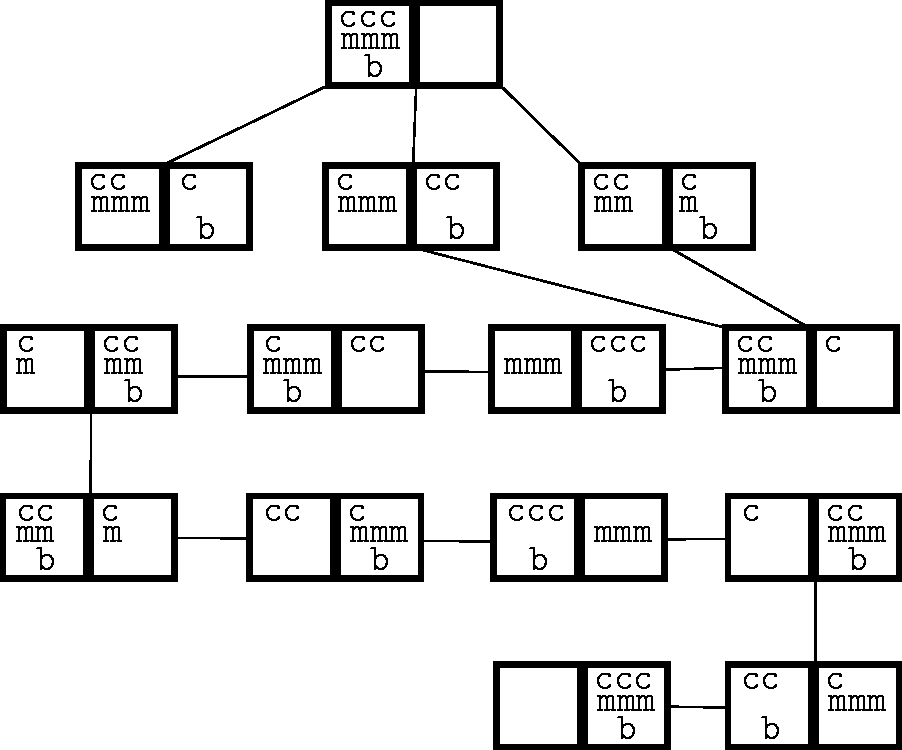
\includegraphics[scale=0.7]{canibales}

\textbf{c)}

Aplicando una búsqueda en profundidad se puede encontrar el siguiente camino hacia el nodo meta:\\
\texttt{cccmmmb |}\\
\texttt{ccmm | bcm}\\
\texttt{ccmmmb | c}\\
\texttt{mmm | bccc}\\
\texttt{cmmmb | cc}\\
\texttt{cm | bccmm}\\
\texttt{ccmmb | cm}\\
\texttt{cc | bcmmm}\\
\texttt{cccb | mmm}\\
\texttt{c | bccmmm}\\
\texttt{ccb | cmmm}\\
\texttt{| bcccmmm}

\section*{Problema 3}

\textbf{a)}

En la primera jugada, el jugador $\times$ puede tirar en cualquiera de las 9 casillas. En la segunda jugada, el jugador $\circ$ puede tirar en el resto de las 8 casillas. En la tercera, $\times$ podrá tirar en el resto de las 7 casillas y así sucesivamente hasta que el juego termine. De aquí se puede notar que una cota superior para el número de juegos que se pueden realizar es 9! = 362880.

Evidentemente, el número real de posibles juegos es menos que eso, pues el juego se termina cuando hay tres fichas del mismo tipo alineadas (es decir, no cualquier nodo hoja será el tablero lleno) y tampoco se están considerando simetrías en los estados del tablero.

\textbf{b)}

\includegraphics[scale=0.6]{gatos1}

\textbf{c)}

Se aplica la función $f(s)$ a cada hoja del árbol. Los valores resultantes de aplicar la función de utilidad se colocan debajo de cada hoja.

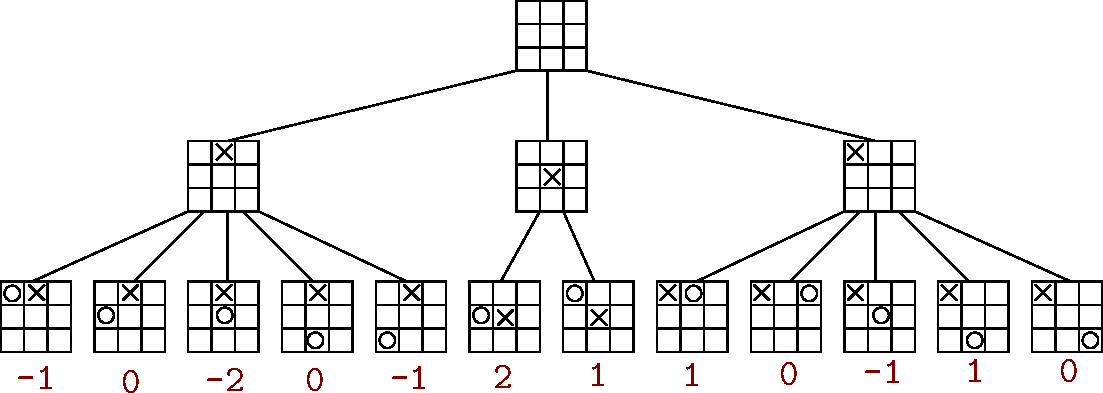
\includegraphics[scale=0.6]{gatos2}

\textbf{d)}

En el siguiente árbol se muestra el valor minimax de cada nodo. Dados esos valores, se determina que el mejor movimiento inicial es tirar al centro del tablero (el siguiente estado donde el valor minimax es 1).

\includegraphics[scale=0.6]{gatos3}

\textbf{e)}

Supongamos que en la poda alfa-beta se realiza una búsqueda en profundidad donde se explora primero al hijo que está más a la izquierda (en este dibujo). Los nodos que no serán evaluados serán las últimas tres hojas (las tres que están más a la derecha), pues se sabe que el valor minimax del padre de esos 3 nodos será menor o igual a 0, pero ya se tiene un nodo a profundidad 1 cuyo valor minimax es 1. Esto quiere decir que el primer movimiento no será tirar a la esquina. En la siguiente figura se encierran en un círculo los nodos que no se van a evaluar.

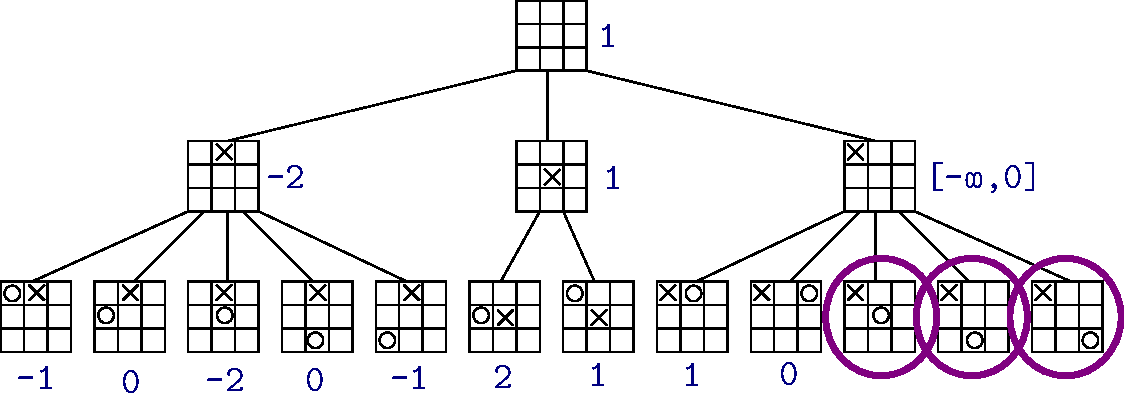
\includegraphics[scale=0.6]{gatos4}

\section*{Problema 4}

Primero, observemos las variables del problema: Colores de casa, Nacionalidades, Dulces, Mascotas, Bebidas. Luego, el dominio de cada variables es:

\begin{itemize}
\item[1.] \textbf{Colores de casas:} roja, marfil, amarilla, verde, azul.
\item[2.] \textbf{Nacionalidades:} ingles, español, noruego, ucraniano, japonés.
\item[3.] \textbf{Dulces:} Hershey, Milky Way, Kit Kat, Snicker, Smartie.
\item[4.] \textbf{Mascotas:} caracoles, perro, zorro, caballo, cebra.
\item[5.] \textbf{Bebidas:} té, agua, café, leche, jugo.
\end{itemize}

Se va a representar el problema con una matriz, donde los colores van en la primera fila, las nacionalidades en la segunda fila, etc. Si se tienen 5 variables para cada casilla y se tienen 5 filas entonces el espacio de búsqueda sin restricciones tiene tamaño $5^5$.

\textbf{a)}

En el siguiente árbol se muestra la búsqueda con backtracking y se coloca un número de acuerdo al orden en el que se exploró cada nodo. En la raíz no se tiene un tablero vacío porque algunos valores ya tienen un lugar fijo.

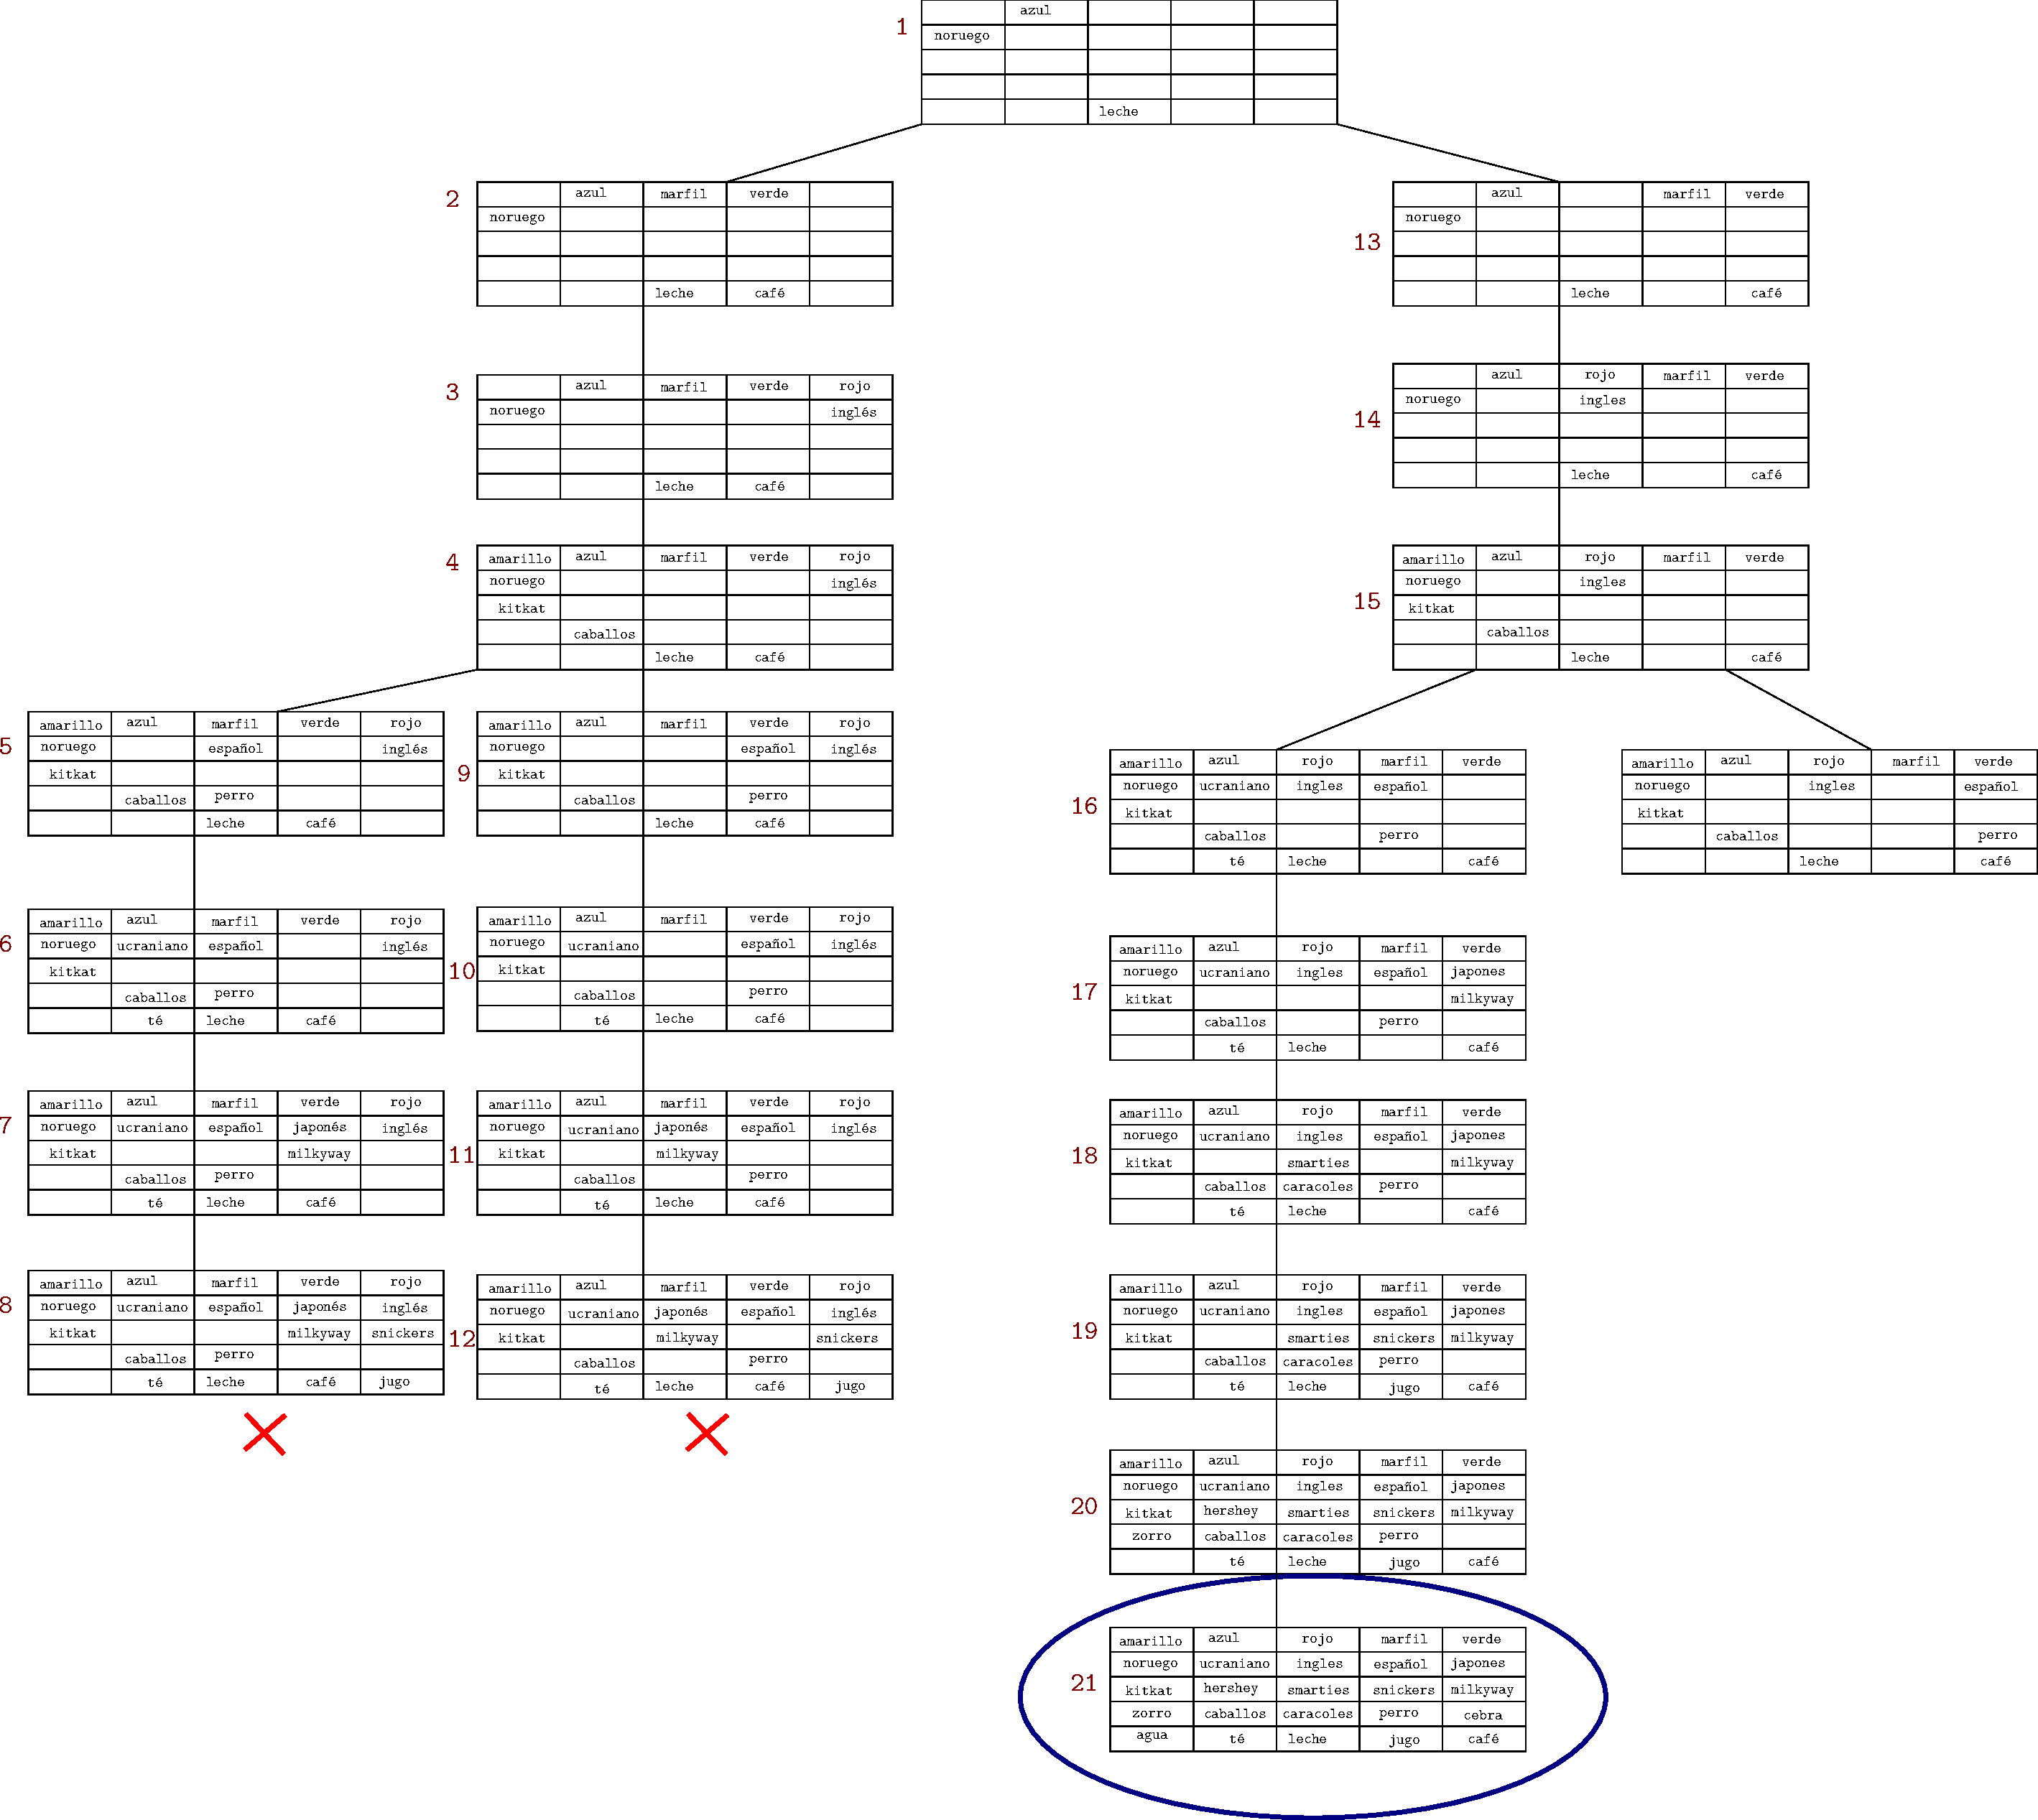
\includegraphics[width=\linewidth]{acertijo}

\textbf{b)}

La cebra vive en la casa verde, que es la que está más a la derecha. El agua se prefiere en la casa amarilla, que es la que está más a la izquierda.

\section*{Problema 5}

\textbf{a)}

Se tienen las variables proposicionales $\{p, q, r, s, t\}$ con el siguiente significado:

\begin{itemize}
\item $p$: un unicornio es mítico.
\item $q$: un unicornio es mortal.
\item $r$: un unicornio es un mamífero.
\item $s$: un unicornio tiene un cuerno.
\item $t$: un unicornio es mágico.
\end{itemize}

El enunciado se puede plantear con lógica proposicional de la siguiente manera:

\begin{itemize}
\item $p \rightarrow \lnot q$: Si un unicornio es mítico, entonces es inmortal.
\item $\lnot p \rightarrow r \land q$: Pero si no es mítico, entonces es un mamífero mortal.
\item $\lnot q \lor r \rightarrow s$: Si el unicornio es inmortal o mamífero entonces tiene un cuerno.
\item $s \rightarrow t$: El unicornio es mágico si tiene un cuerno.
\end{itemize}

Así que se tiene el siguiente conjunto de fórmulas ($\Gamma$):

$\Gamma = \{p \rightarrow \lnot q, \lnot p \rightarrow r \land q, \lnot q \lor r \rightarrow s, s \rightarrow t\}$

\textbf{b)}

Primero se transformarán las fórmulas del conjunto $\Gamma$ a sus equivalentes en forma normal conjuntiva.

\begin{itemize}
\item $p \rightarrow \lnot q \equiv \lnot p \lor \lnot q$
\item $\lnot p \rightarrow r \land q \equiv p \lor (r \land q) \equiv (p \lor r) \land (p \lor q)$
\item $\lnot q \lor r \rightarrow s \equiv \lnot (\lnot q \lor r) \lor s \equiv (q \land \lnot r) \lor s \equiv (q \lor s) \land (\lnot r \lor s)$
\item $s \rightarrow t \equiv \lnot s \lor t$
\end{itemize}

Así, se tiene el nuevo conjunto de fórmulas $\Gamma = \{\lnot p \lor \lnot q, p \lor r, p \lor q, q \lor s, \lnot r \lor s, \lnot s \lor t\}$.

La variable $p$ es la que representa si un unicornio es mítico. Si el conjunto $\Gamma \cup \{\lnot p\}$ es insatisfacible, entonces el unicornio es mítico; por otro lado, si es satisfacible entonces el unicornio no es mítico.

Tomemos la siguiente asignación de valores a las variables:

\begin{tabular}{|c|c|c|c|c|}
\hline
$p$ & $q$ & $r$ & $s$ & $t$ \\ \hline
 0  &  1  &  1  &  1  &  1  \\ \hline  
\end{tabular}

Con ese estado se hace verdadero el conjunto de fórmulas $\Gamma \cup \{\lnot p\}$ y por lo tanto es satisfacible. Con esto se concluye que el unicornio no es mítico.

\textbf{c)}

Si el conjunto $\Gamma \cup \{\lnot t\}$ es insatisfacible entonces el unicornio sí es mágico. Se procederá a hacer resolución binaria con el conjunto de fórmulas $\Gamma \cup \{\lnot t\}$.

\begin{itemize}
\item[1)] $\lnot p \lor \lnot q$
\item[2)] $p \lor r$
\item[3)] $p \lor q$
\item[4)] $q \lor s$
\item[5)] $\lnot r \lor s$
\item[6)] $\lnot s \lor t$
\item[7)] $\lnot t$
\item[8)] $\lnot s$ Res(6,7)
\item[9)] $\lnot r$ Res(8,5)
\item[10)] $p$ Res(2,9)
\item[11)] $\lnot q$ Res(1,10)
\item[12)] $s$ Res(4,11)
\item[13)] $\square$ Res(8,12)
\end{itemize}

Como se obtiene una cláusula vacía, el conjunto $\Gamma \cup \{\lnot t\}$ es insatisfacible y se concluye que el unicornio sí es mágico.

\textbf{d)}

Si el conjunto $\Gamma \cup \{\lnot s\}$ es insatisfacible entonces el unicornio sí tiene un cuerno. Se procederá a hacer resolución binaria con el conjunto de fórmulas $\Gamma \cup \{\lnot s\}$.

\begin{itemize}
\item[1)] $\lnot p \lor \lnot q$
\item[2)] $p \lor r$
\item[3)] $p \lor q$
\item[4)] $q \lor s$
\item[5)] $\lnot r \lor s$
\item[6)] $\lnot s \lor t$
\item[7)] $\lnot s$
\item[8)] $\lnot r$ Res(5,7)
\item[9)] $q$ Res(4,7)
\item[10)] $p$ Res(2,8)
\item[11)] $\lnot q$ Res(1,10)
\item[12)] $\square$ Res(9,11)
\end{itemize}

Se obtuvo la cláusula vacía, así que se concluye que el unicornio sí tiene un cuerno.

\section*{Problema 6}

\textbf{Constantes}: tomate, carne, John, Mary, OmegaMart, $\mathbb{Q}$.

En este caso, $\mathbb{Q}$ es el conjunto de números racionales.

\textbf{Funciones}: $fkt(x) = 6x$.

\textbf{Predicados} (y su significado):

\begin{itemize}
\item Adulto($x$) := $x$ es un adulto.
\item Niño($x$) := $x$ es un niño.
\item Efectivo($x$) := $x$ lleva efectivo.
\item Tarjeta($x$) := $x$ lleva tarjeta.
\item Compra($x, y$) := $x$ compra $y$.
\item Kg($x, y$) := Hay $y$ kilogramos de $x$.
\item Cantidad($x, y$) := Hay $y$ de $x$.
\item Menor($x, y$) := $x$ es menor que $y$.
\item Ir($x, y$) := $x$ va a $y$.
\item Ver($x, y$) := $x$ ve a $y$.
\item Producir($x, y$) := $x$ se produce en $y$.
\item Dinero($x, y$) := $x$ tiene $y$ pesos.
\item Super($x$) := $x$ es supermercado.
\item Comer($x, y$) := $x$ come $y$.
\end{itemize}

\textbf{Conjunto de fórmulas}

\begin{itemize}
\item Ir(John, OmegaMart) $\land$ Compra(John, tomate) $\land$ Compra(John, carne) $\land$ Kg(tomate, 1/2) $\land$ Kg(carne, 1/4)
\item Adulto(John)
\item Adulto(Mary)
\item Super(OmegaMart)
\item $\lnot$ Niño(John)
\item $\forall$ Kg(tomates, $x$) $\rightarrow$ Cantidad(tomates, $fkt(x)$) (estoy suponiendo que 1 kg de tomates son 6 tomates).
\item $\forall x \forall y \forall z$ Ir($x, y$) $\land$ Ir($z, y$) $\rightarrow$ Ver($x, z$)
\item $\forall x \forall y$ Ver($x, y$) $\rightarrow$ Ver($y, x$)
\item $\forall x$ Super($x$) $\rightarrow$ $\lnot$ Producir(tomate, $x$)
\item Comer(John, tomate)
\item $\forall x \forall y$ Adulto($x$) $\land$ Super($y$) $\land$ Ir($x, y$) $\rightarrow$ Efectivo($x$) $\lor$ Tarjeta($x$)
\item $\forall x \forall y \forall z \forall w$ Adulto($x$) $\land$ Super($y$) $\land$ Ir($x, y$) $\land$ Dinero($x, z$) $\rightarrow$ Dinero($x, w$) $\land$ Menor($w, z$)
\end{itemize}

\end{document}

